\subsection{Portas Lógicas}
\label{sec:portas}

Portas lógicas são circuitos eletrônicos que utilizam transistores para realizar operações matemáticas sob Álgebra Booleana. Elas recebem sinais binários de entrada e processam uma única saída lógica.

\subsubsection{Not}

A porta lógica NOT (inversora) é responsável por inverter o sinal de entrada: quando a entrada é 1, a saída é 0, e vice-versa.

\begin{align*}
	y &= \neg x
\end{align*}

\begin{center}
\begin{tabular}{c|c}
$x$&$y$\\
\hline
$0$&$1$\\
$1$&$0$\\

\end{tabular}
\end{center}

Em implementações mais simples, a porta NOT pode ser construída com um único transistor e resistores. No entanto, em circuitos digitais modernos, utiliza-se a tecnologia CMOS, que emprega dois transistores: um do tipo PMOS e outro do tipo NMOS.

Nessa configuração, os transistores atuam de forma complementar: quando o sinal de entrada é baixo, o transistor PMOS conduz e conecta a saída ao nível lógico alto (Vcc); quando o sinal de entrada é alto, o transistor NMOS conduz e conecta a saída ao nível lógico baixo (GND).

\begin{figure}[H]
    \centering
    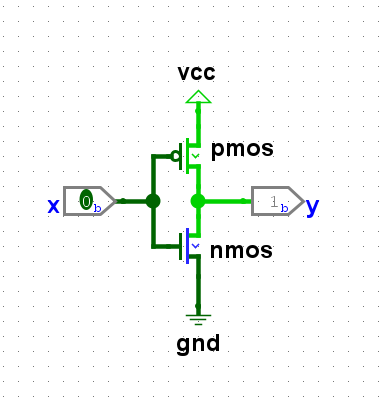
\includegraphics[width=0.6\linewidth]{images/not-circuit.png}
    \caption{Circuito de uma porta NOT}
    \label{fig:not-circuit}
\end{figure}

Utilizamos esta notação para esse circúito:

\begin{figure}[H]
   	\centering
   	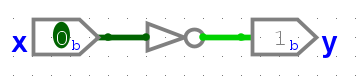
\includegraphics[width=0.6\linewidth]{images/not-gate.png}
  	 \caption{Notação Not}
   	\label{fig:not-gate}
	%{\footnotesize Fonte: \url{https://autoctrls.com/datasheet-transistor/}}
\end{figure}


\subsubsection{OR}

A porta lógica OR produz saída 1 quando pelo menos uma das entradas está em nível lógico 1.

\begin{align*}
    x = a \lor b
\end{align*}

\begin{center}
\begin{tabular}{cc|c}
$a$ & $b$ & $x$ \\
\hline
0 & 0 & 0 \\
0 & 1 & 1 \\
1 & 0 & 1 \\
1 & 1 & 1 \\
\end{tabular}
\end{center}

Uma implementação clássica da porta OR pode ser derivada a partir da porta NOR (Not Or). Em CMOS, a NOR é construída com transistores PMOS em série no pull-up network e NMOS em paralelo no pull-down network. A função OR pode então ser obtida pela inversão da saída da NOR.

\begin{figure}[H]
    \centering
    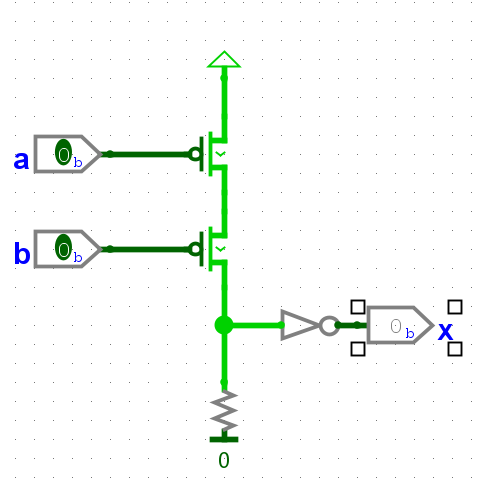
\includegraphics[width=0.6\linewidth]{images/or-circuit.png}
    \caption{Implementação CMOS pull down de uma porta OR}
    \label{fig:or-circuit}
\end{figure}

\begin{figure}[H]
    \centering
    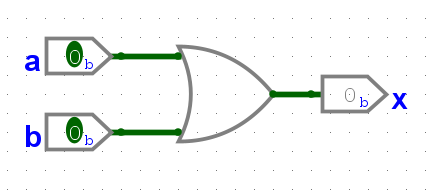
\includegraphics[width=0.6\linewidth]{images/or-gate.png}
    \caption{Símbolo lógico da porta OR}
    \label{fig:or-gate}
\end{figure}

\subsubsection{And}

 A porta And resulta em saída 1 se e somente se as duas entradas estiverem no estado lógico 1. 

\begin{align*}
	x = b \land a
\end{align*}

\begin{center}
\begin{tabular}{cc|c}
$a$&$b$&$x$\\
\hline
$0$&$0$&$0$\\
$0$&$1$&$0$\\
$1$&$0$&$0$\\
$1$&$1$&$1$\\

\end{tabular}
\end{center}

A implementação direta da porta AND em CMOS não é a forma mais eficiente. Na prática, constrói-se a porta NAND (Not And) utilizando transistores NMOS em série no pull-down e PMOS em paralelo no pull-up. Em seguida, aplica-se uma inversão para obter a função AND.

\begin{figure}[H]
   	\centering
   	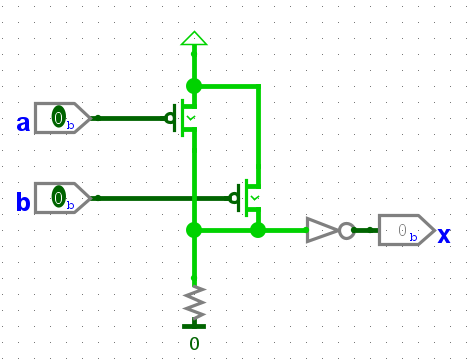
\includegraphics[width=0.6\linewidth]{images/and-circuit.png}
  	 \caption{Circuito CMOS pull-down de uma porta And}
   	\label{fig:or-circuit}
	%{\footnotesize Fonte: \url{https://autoctrls.com/datasheet-transistor/}}
\end{figure}

Utilizamos esta notação para esse circúito:

\begin{figure}[H]
   	\centering
   	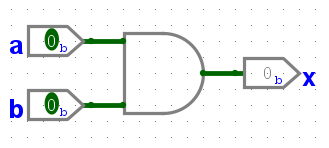
\includegraphics[width=0.6\linewidth]{images/and-gate.png}
  	 \caption{Notação And}
   	\label{fig:not-gate}
	%{\footnotesize Fonte: \url{https://autoctrls.com/datasheet-transistor/}}
\end{figure}

\subsubsection{XOR}

A porta lógica XOR (Exclusive OR) produz saída 1 quando as entradas são diferentes, e 0 quando são iguais.

\begin{align*}
    x = a \oplus b
\end{align*}

\begin{center}
\begin{tabular}{cc|c}
$a$ & $b$ & $x$ \\
\hline
0 & 0 & 0 \\
0 & 1 & 1 \\
1 & 0 & 1 \\
1 & 1 & 0 \\
\end{tabular}
\end{center}

Também pode ser expressa como:

\begin{align*}
    x = (a \land \neg b) \lor (\neg a \land b)
\end{align*}

%Diferentemente das portas AND e OR, a XOR não é diretamente implementada de forma eficiente em CMOS com uma única estrutura pull-up/pull-down simples. Em vez disso, sua implementação é tipicamente construída a partir da combinação de portas básicas, derivada da manipulação algébrica demonstrada acima.

\begin{figure}[H]
    \centering
    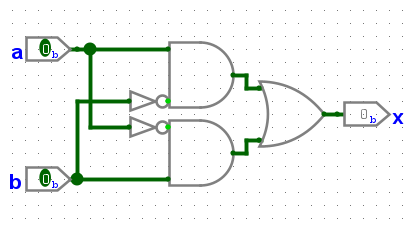
\includegraphics[width=0.6\linewidth]{images/xor-circuit.png}
    \caption{Implementação lógica de uma porta XOR}
    \label{fig:xor-circuit}
\end{figure}

\begin{figure}[H]
    \centering
    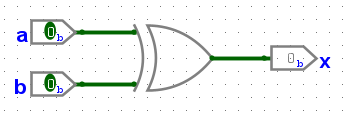
\includegraphics[width=0.6\linewidth]{images/xor-gate.png}
    \caption{Símbolo lógico da porta XOR}
    \label{fig:xor-gate}
\end{figure}

%Alternativamente, em circuitos CMOS otimizados, a XOR pode ser implementada com redes de transmissão (\textit{transmission gates}), reduzindo o número de transistores e melhorando o desempenho, entretanto, para o presente documento, isso serve somente à título de curiosidade.

%\begin{figure}[H]
%    \centering
%    \includegraphics[width=0.6\linewidth]{images/xor-gate-cmos.png}
%    \caption{Símbolo lógico da porta XOR}
%    \label{fig:xor-gate}
%\end{figure}W

A porta XOR é fundamental na implementação de circuitos aritméticos, especialmente somadores binários (half-adder e full-adder), sendo responsável pelo cálculo do bit de soma.